% Minor ticks above the last major tick appear only when the upper limit is at
% least half a major step beyond it (behaviour Z13, found by the generator fuzz):
% y limits [2.79, 8.91], majors 4, 6, 8: none above 8; x [0.3, 4.6]: minors up to 4.5.
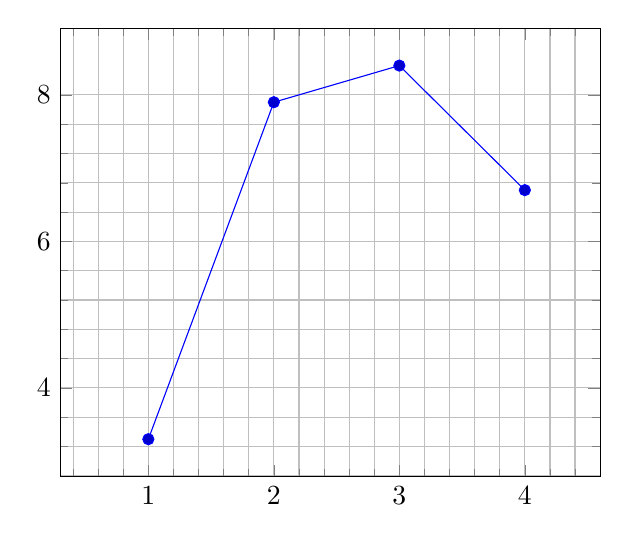
\begin{tikzpicture}
\begin{axis}[minor tick num=4, xmin=0.3, xmax=4.6, grid=both]
\addplot coordinates {(1,3.3) (2,7.9) (3,8.4) (4,6.7)};
\end{axis}
\end{tikzpicture}
